\section{Validation and interpretation of PineAPPL grids}
\label{sec:results}

In this section we demonstrate the capabilities of \textsc{PineAPPL} by
computing fast-interpolation grids, accurate to NLO QCD and NLO QCD+EW,
for a representative set of processes in which EW corrections may have a
sizeable effect on the accuracy of the theoretical predictions.
In order to consider some realistic kinematics for these
processes, we resort to measurements commonly devised for inclusion in PDF
fits. Our aim is twofold. First, we want to validate the results
obtained with \textsc{PineAPPL}; second, we want to assess the
impact of the EW corrections for usual experimental setups. We describe, first,
the processes and measurements that we consider, then the computational
settings that we adopt, and finally the results that we obtain.

\subsection{Processes and measurements}
\label{subsec:processes_and_measurements}

We focus on the following three processes: Drell--Yan lepton-pair production,
top-quark pair production, and Z-boson (lepton-pair) production with non-zero
transverse momentum in proton-proton collisions. For each of these processes,
we consider the following measurements.

\paragraph{Drell--Yan lepton pair production.}
We select the distribution, single-differential in the invariant mass of the
lepton pair, $M_{\ell \bar\ell}$, measured by the ATLAS experiment at a centre-of-mass
energy of \SI{7}{\tera\electronvolt} in the high-mass region
($M_{\ell\bar\ell}>\SI{116}{\giga\electronvolt}$)~\cite{Aad:2013iua}.
We also select the distributions, double-differential in the rapidity and in
the invariant mass of the lepton pair, $y_{\ell\bar\ell}$ and $M_{\ell\bar\ell}$,
measured by the CMS experiment at a centre-of-mass energy of
\SI{7}{\tera\electronvolt}~\cite{Chatrchyan:2013tia}.
These measurements are currently included as standard in the
NNPDF3.1~\cite{Ball:2017nwa} and MMHT2014~\cite{Harland-Lang:2014zoa} PDF sets,
although with appropriate kinematic cuts that remove the bins at the largest
values of invariant mass, where EW corrections become sizeable. As explained in
section~\ref{sec:pineappl-example}, should PI contributions be taken into account,
the process has a single LO, $\mathcal{O}(\alpha^2)$; at NLO, the
QCD contribution is $\mathcal{O}(\alphas\alpha^2)$, while the EW contribution
is $\mathcal{O}(\alpha^3)$. The latter is not included in the NLO
QCD computation, but it is in the NLO QCD+EW computation. Mixed QCD-EW
corrections occur only at NNLO, and are therefore not considered here.
EW corrections for this process were computed in
refs.~\cite{Baur:2001ze,Dittmaier:2009cr}. The process receives contributions
from 12 (34) parton luminosities at NLO QCD (NLO QCD+EW),
see appendix~\ref{app:lumis} for details.

\paragraph{Top-quark pair production.}
We select the distributions, single-differential in either the transverse
momentum of the top quark, $p_\mathrm{T}^\mathrm{t}$, or the invariant mass of the top-quark
pair, $m_{\mathrm{t}\bar{\mathrm{t}}}$, measured by the ATLAS and CMS experiments at a centre-of-mass
energy of \SI{8}{\tera\electronvolt}~\cite{Aad:2015mbv,Khachatryan:2015oqa}. These measurements have
been extensively studied in the context of PDF fits in
refs.~\cite{Czakon:2016olj,Bailey:2019yze,Amoroso:2020lgh,Kadir:2020yml}, and
included by default in the CT18~\cite{Hou:2019efy} analysis.
Because EW corrections are significantly smaller for distributions differential
in the rapidity of either the top quark or the top-quark
pair~\cite{Czakon:2017wor}, these distributions were preferred for inclusion
in the NNPDF3.1 analysis~\cite{Ball:2017nwa}. The process receives
pure QCD contributions at LO, $\mathcal{O}(\alphas^2)$, and
at NLO, $\mathcal{O}(\alphas^3)$. They make up the NLO QCD
computation. The NLO QCD+EW computation includes the LO contribution
$\mathcal{O}(\alphas\alpha)$ and the NLO contributions
$\mathcal{O}(\alphas^2\alpha)$ and $\mathcal{O}(\alphas\alpha^2)$.
We do not consider the LO contribution $\mathcal{O}(\alpha^2)$ and the
corresponding higher-order EW correction. EW corrections for this process
were computed in refs.~\cite{Bernreuther:2010ny,Hollik:2011ps,Kuhn:2011ri,Bernreuther:2012sx,Pagani:2016caq,Czakon:2017wor,Czakon:2017lgo,Czakon:2017mmr,Czakon:2019bcq,Czakon:2019txp}. The process receives contributions from
6 (36) parton luminosities at NLO QCD (NLO QCD+EW),
see appendix~\ref{app:lumis} for details.

\paragraph{Z-boson production with non-zero transverse momentum.}
We select the distribution, single-differential in the transverse momentum of
the Z boson, $p_\mathrm{T}^\mathrm{Z}$, measured by the CMS experiment at a centre-of-mass
energy of \SI{13}{\tera\electronvolt}~\cite{Sirunyan:2019bzr}. So far, this measurement has not been
included in any PDF determination. Because it has sub-percent uncertainties,
EW corrections are expected to be essential in order to achieve a good
description of it, and to constrain accurately the PDFs. Analogous measurements,
from the ATLAS~\cite{Aad:2015auj} and CMS~\cite{Khachatryan:2015oaa}
experiments at a centre-of-mass energy of \SI{8}{\tera\electronvolt}, were partly included (upon
selection of an appropriate kinematic cut that excluded bins with large EW
corrections) in the NNPDF3.1 PDF set~\cite{Ball:2017nwa} and in variants of
the CT18 PDF set~\cite{Hou:2019efy}. In the QCD computation, we consider a
single LO contribution $\mathcal{O}(\alphas\alpha^2)$ and a single NLO
contribution $\mathcal{O}(\alphas^2\alpha^2)$. In the NLO QCD+EW computation,
we supplement these with the LO and NLO EW corrections,
$\mathcal{O}(\alpha^3)$ and $\mathcal{O}(\alpha^4)$, and with the NLO
QCD-EW mixed correction, $\mathcal{O}(\alphas\alpha^3)$. EW corrections for
this process were computed in
refs.~\cite{Kuhn:2005az,Denner:2011vu,Hollik:2015pja,Kallweit:2015dum}.
The process receives contributions from 100 (165) parton luminosities,
see appendix~\ref{app:lumis} for details.

\subsection{Computational settings}
\label{subsec:computational_settings}

We generate each process by means of the Universal FeynRules Output
(UFO)~\cite{Degrande:2011ua} model {\tt loop\_qcd\_qed\_sm\_Gmu},
included as standard in {\sc MG5\_aMC}. It contains the UV and $R_2$
counterterms relevant to NLO QCD and EW corrections, the latter in the
$\overline{G}_\mu$ scheme. The model features five massless quark flavours,
sets the CKM matrix equal to the identity, and is compatible with the usage of
the complex mass (CM) scheme for all massive particles, see
ref.~\cite{Frederix:2018nkq} for details. We use this scheme
for all processes that do not involve stable top quarks in the final state.
The photon is always considered as part of the proton in the initial state and
of any hadronic jet produced in the final state: PI effects and EW corrections
are therefore treated on the same footing. We use a PDF set that contains a
consistently defined photon PDF, namely
{\tt NNPDF31\_nlo\_as\_0118\_luxqed}~\cite{Bertone:2017bme}. We evaluate the PDF
uncertainty associated to the theoretical predictions a posteriori, that is,
we convolve the fast-interpolation grid generated with {\sc PineAPPL} with
each member in the PDF set, and we compute the associated standard deviation.

The central values of the renormalisation and factorisation scales, $\mu_\mathrm{R}$ and
$\mu_\mathrm{F}$, are chosen, for each process, as follows. In the case of Drell--Yan
lepton pair production, we use the fixed scale $\mu_\mathrm{R}=\mu_\mathrm{F}=M_\mathrm{Z}$, where $M_\mathrm{Z}$ is
the mass of the Z boson, for the ATLAS measurement, and the scale
$\mu_\mathrm{R}=\mu_\mathrm{F}=M_{\ell\bar\ell}$, where $M_{\ell\bar\ell}$ is the central value of each
invariant mass bin, for the CMS measurement.
In the case of top-quark pair production, we use the dynamic scales
$\mu_\mathrm{R}=\mu_\mathrm{F}=\sqrt{m_\mathrm{t}^2+(p_\mathrm{T}^\mathrm{t})^2}{\Big /}2$ for the distribution differential
in the transverse momentum of the top quark, and $\mu_\mathrm{R}=\mu_\mathrm{F}=H_\mathrm{T}/4$ for the
distribution differential in the invariant mass of the top-quark pair, where
$H_\mathrm{T}=\sqrt{m_\mathrm{t}^2+(p_\mathrm{T}^\mathrm{t})^2}+\sqrt{m_\mathrm{t}^2+(p_\mathrm{T}^{\bar{\mathrm{t}}})}$, with $m_\mathrm{t}$,
$p_\mathrm{T}^\mathrm{t}$ and $p_\mathrm{T}^{\bar{\mathrm{t}}}$ the mass of the top quark and the transverse momenta
of the top and antitop quarks, respectively. These choices were demonstrated
to maximise the convergence of the perturbative expansion~\cite{Czakon:2016dgf}.
In the case of Z-boson production with non-zero transverse momentum, we use
$\mu_\mathrm{R}=\mu_\mathrm{F}=M_\mathrm{Z}$. In order to estimate the missing higher-order uncertainty,
we allow the events to be reweighted in the Monte Carlo generation upon scale
variations. To this purpose, we use the default \textsc{MG5\_aMC}
implementation, whereby the factorisation and renormalisation scales
are varied down to a factor $1/2$ and up to a factor $2$, and the envelope
from the nine-point scale variations is constructed. However, we note that
\textsc{PineAPPL} allows the user to determine the envelope with any point
prescription, see appendix~\ref{app:pineappl-demo} for an example.

The values of the relevant physical parameters are chosen as
\begin{equation}
\begin{aligned}
M_\mathrm{W} &= \SI{80}{\giga\electronvolt} \text{,} \quad &
M_\mathrm{Z} &= \SI{91.176}{\giga\electronvolt} \text{,} \quad &
m_\mathrm{t} &= \SI{172.5}{\giga\electronvolt} \text{,} \quad \\
\Gamma_\mathrm{W} &= \SI{2.09}{\giga\electronvolt} \text{,} &
\Gamma_\mathrm{Z} &= \SI{2.50}{\giga\electronvolt} \text{,}
\end{aligned}
\label{eq:parameters}
\end{equation}
where $M_\mathrm{W}$, $M_\mathrm{Z}$ and $m_\mathrm{t}$ are the values of the W-boson, Z-boson, and
top quark masses, respectively, and $\Gamma_\mathrm{W}$ and $\Gamma_\mathrm{Z}$ are the width of
the W boson and of the Z boson, respectively. The value of the strong
coupling is chosen consistently with the PDF set, $\alphas(M_\mathrm{Z})=0.118$.
When relevant, final-state photons and massless charged fermions (leptons and light quarks) are recombined together 
if they satisfy the condition $\Delta R_{f \gamma} < 0.1$. In this case the
sum of their momenta is assigned to the charged fermion, and the photon is removed
from the event. Kinematics observables and cuts are defined starting from recombined momenta. In 
case we would have been interested also to jet-related observables,
photons surviving the recombination should have to be clustered together with coloured
partons.\footnote{For issues related to the definition of jets in presence of EW corrections,
    see refs.~\cite{Frederix:2016ost,Denner:2019zfp}} 
    
Finally, we implement the kinematic cuts specified in the corresponding
experimental analyses. In the case of high-mass Drell--Yan lepton pair
production at \SI{7}{\tera\electronvolt} measured by ATLAS, we require $p_\mathrm{T}^\ell>\SI{25}{\giga\electronvolt}$,
$|\eta_\ell|<2.5$ and $\SI{116}{\giga\electronvolt}<M_{\ell\bar\ell}<\SI{1500}{\giga\electronvolt}$ for the transverse
momentum and the rapidity of each lepton and for the invariant mass of the
lepton pair, respectively. In the case of double-differential Drell--Yan
lepton-pair production
at \SI{7}{\tera\electronvolt} measured by CMS, we require $p_\mathrm{T}^{\ell_1}>\SI{14}{\giga\electronvolt}$, $p_\mathrm{T}^{\ell_2}>\SI{9}{\giga\electronvolt}$,
$|\eta_\ell|<2.4$, $|\eta_{\ell\bar\ell}|<2.4$ and $\SI{20}{\giga\electronvolt}<M_{\ell\bar\ell}<\SI{1500}{\giga\electronvolt}$
for the transverse momentum and the rapidity of each lepton, and for the
rapidity and the invariant mass of the lepton pair. In the case of Z-boson
production with non-zero transverse momentum at \SI{13}{\tera\electronvolt} measured by CMS, we
require $p_\mathrm{T}^\ell>\SI{25}{\giga\electronvolt}$, $|\eta_\ell|<2.4$,
$M_\mathrm{Z}-\SI{15}{\giga\electronvolt}<M_{\ell\bar\ell}<M_\mathrm{Z}+\SI{20}{\giga\electronvolt}$,
$|\eta_{\ell\bar\ell}|<2.4$ and $\SI{20}{\giga\electronvolt}<p_\mathrm{T}^{\ell\bar\ell}<\SI{1500}{\giga\electronvolt}$ for the
transverse momentum and rapidity of each lepton, and for the invariant mass,
rapidity and transverse momentum of the lepton pair.

\subsection{Numerical results}
\label{subsec:numerical_results}

For each of the measurements discussed in
section~\ref{subsec:processes_and_measurements}, we compute the expectation
value of the corresponding observable for each kinematic bin in two different
ways: directly, by means of \textsc{MG5\_aMC}, and a posteriori, by convolving
the fast-interpolation grid produced by \textsc{PineAPPL} with the PDF set
specified in section~\ref{subsec:computational_settings}. In the following, we
will refer to the first result as the MC result, and to the second as
the \textsc{PineAPPL} result. We repeat the computation for theories accurate
to NLO QCD and to NLO QCD+EW, respectively. The corresponding orders of the
strong and electroweak couplings that we consider have been specified in
section~\ref{subsec:processes_and_measurements}. In each case, we determine the
PDF uncertainty (coming from the PDF ensemble), the scale uncertainty (coming
from variations of the factorisation and renormalisation scales), and the Monte
Carlo uncertainty (coming from the finite number of events generated). In this
last respect, we consider by default high-statistics computations, whereby we
require a relative Monte Carlo precision of a fraction of per mille. While
this choice does not affect the validation of the \textsc{PineAPPL} result
against the MC result, it ensures that the statistical uncertainty of
the computation remains negligible in comparison to the PDF and scale
uncertainties, as we will explicitly demonstrate. This is a desirable feature
to correctly interpret the size of the EW corrections.

Our goal is indeed twofold. On the one hand, we aim to validate the
interpolation grids generated with \textsc{PineAPPL}: to this purpose we shall
verify that the MC and the \textsc{PineAPPL} results are identical up to
numerical inaccuracies due to the grid interpolation. This equivalence must
hold for any choice of renormalisation and factorisation scale. On the other
hand, we aim to study the size of the EW corrections, in particular with
respect to the kinematics of each process, and to three kinds of uncertainties:
the PDF uncertainty, the scale uncertainty, and the uncertainty of the
experimental data.

We present these comparisons in
figures~\ref{fig:atlaszhighmass49fb}--\ref{fig:cmsZ13TeV} for each of the processes
and data sets outlined in section~\ref{subsec:processes_and_measurements}.
The format of the plots is the same across all figures. The first panel
displays the relative difference (in per mille) between the {\sc PineAPPL} and
the MC results for the central, upper and lower scale choices, for
theories accurate to both NLO QCD and NLO QCD+EW. The following three panels
present the theoretical predictions, accurate to either NLO QCD or NLO QCD+EW,
always normalised to the former; on top of the theoretical predictions, the
PDF uncertainty, the scale uncertainty and the Monte Carlo uncertainty are
displayed in turn. The relative uncertainty of the experimental data is
also shown for comparison. We shall now discuss the results for each
process and data set.

\paragraph{Drell--Yan lepton pair production.} 

We first consider the single-differential measurement at a high lepton-pair
invariant mass performed by the ATLAS experiment at \SI{7}{\tera\electronvolt}.
From figure~\ref{fig:atlaszhighmass49fb} we immediately
observe that the validation of the \textsc{PineAPPL} result against the MC
result is successful. The relative difference between the two is of the order
$0.1\tcperthousand$ at most, with negligible fluctuations across different
invariant mass bins. The agreement is similarly good irrespective of the
perturbative accuracy of the theory (NLO QCD or NLO QCD+EW) or of the scale
choice.

%-------------------------------------------------------------------------------
\begin{figure}[!t]
    \centering
    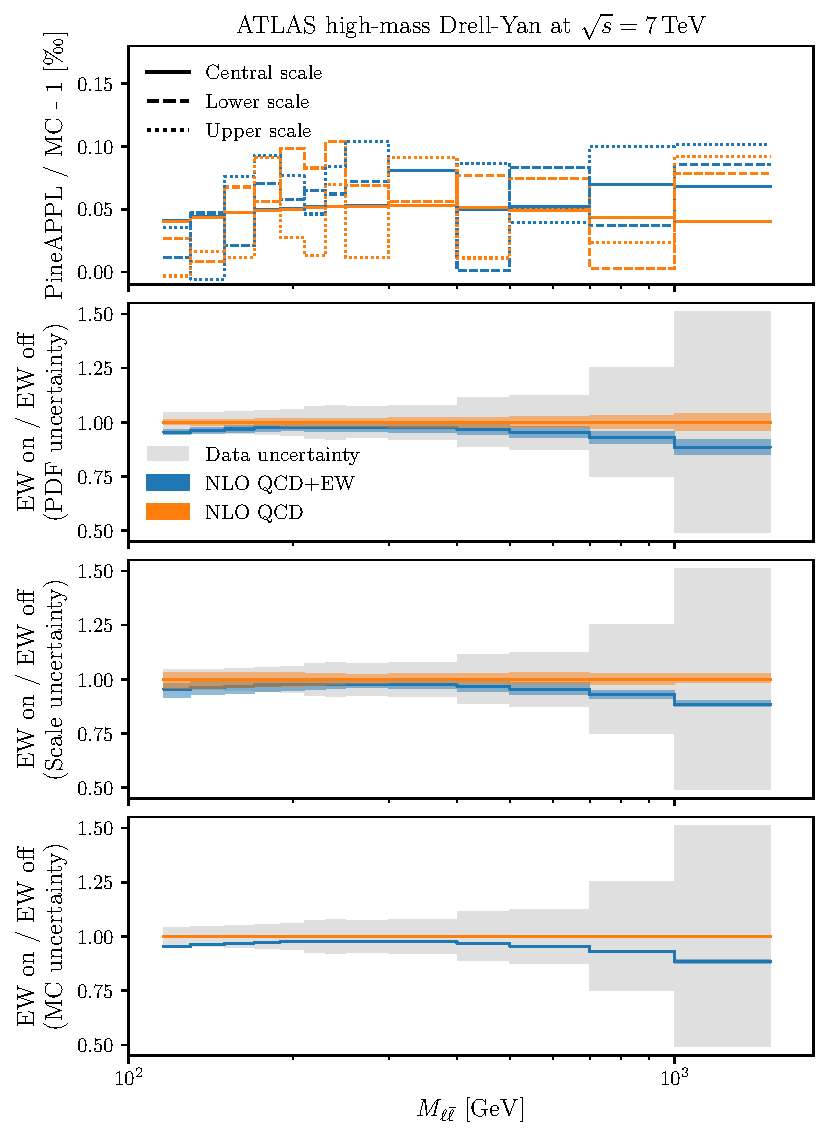
\includegraphics[width=0.5\textwidth]{figures/pineappl_ATLASZHIGHMASS49FB}
    \caption{Validation and test of the \textsc{PineAPPL} grid for the ATLAS
      high-mass Drell--Yan lepton pair measurement in the high-mass region at
      a centre-of-mass energy of \SI{7}{\tera\electronvolt}~\cite{Aad:2013iua}. The first panel
      displays the relative difference (in per mille) between the {\sc PineAPPL}
      and the MC results for the central, upper and lower scale choices,
      for theories accurate to both NLO QCD and NLO QCD+EW. The second, third
      and fourth panels present the theoretical predictions, accurate to either
      NLO QCD or NLO QCD+EW, always normalised to the former; on top of the
      theoretical predictions, the PDF uncertainty, the scale uncertainty and
      the Monte Carlo uncertainty are displayed in turn. The relative
      uncertainty of the experimental data is also shown for comparison.}
    \label{fig:atlaszhighmass49fb}
\end{figure}
%-------------------------------------------------------------------------------

The measurement is mainly driven by $\mathrm{q}\bar{\mathrm{q}}$ scattering: specifically, the
leading (next-to-leading) contribution comes from a $\mathrm{u}\bar{\mathrm{u}}$ ($\mathrm{d}\bar{\mathrm{d}}$)
parton luminosity, which accounts for about \SI{55}{\percent} (\SI{49}{\percent}) of the cross section
for the lowest invariant mass bins, and \SI{68}{\percent} (\SI{22}{\percent}) for the largest invariant
mass bins. The PI contribution raises from about \SI{1.3}{\percent} in the lowest bin to
about \SI{3.6}{\percent} in the highest bin. Overall, the EW corrections range between \SI{5}{\percent}
around $M_{\ell\bar\ell}\sim \SI{150}{\giga\electronvolt}$, \SIrange{2}{3}{\percent} for intermediate invariant mass
values, $\SI{150}{\giga\electronvolt}\lesssim M_{\ell\bar\ell}\lesssim \SI{700}{\giga\electronvolt}$, and
\SIrange{15}{20}{\percent} for the largest invariant mass bin, $M_{\ell\bar\ell}>\SI{1000}{\giga\electronvolt}$,
see figure~\ref{fig:atlaszhighmass49fb}. For this reason, the data points with
$M_{\ell\bar\ell}>\SI{210}{\giga\electronvolt}$ were not included in the NNPDF3.1
analysis~\cite{Ball:2017nwa}.

The NLO QCD+EW corrections always lead to a reduction of the cross section in
comparison to the NLO QCD prediction. The size of this shift is comparable to
the data uncertainty at small values of $M_{\ell\bar\ell}$, and rapidly becomes
negligible with respect to it as the value of the invariant mass increases
and the data uncertainty blows up. This fact suggests a couple of observations
in light of the inclusion of EW corrections in a fit of PDFs. First, the
description of the more precise bins in the low invariant mass range is likely
to change, and will possibly become more accurate should the inclusion of EW
corrections improve the data/theory agreement. Second, the kinematic cut that
excludes any data point at large $M_{\ell\bar\ell}$ can be safely removed: any
shift in the predictions induced by the more accurate NLO QCD+EW theory is
likely to be easily accommodated by the large data uncertainty.

In comparison to the PDF uncertainty, the size of the EW corrections is
always larger, especially at the boundaries of the distribution. This fact
suggests that, once included in a global fit, EW corrections could recast the
relative weight of each data set included in the fit, and possibly lead to
an improvement in their overall description. In comparison to the scale
uncertainty, the size of the EW correction is similar, except for the four bins
at the largest invariant mass, where the latter is significantly larger than
the former. The size of the scale variation is the same for the QCD and the
QCD+EW theories. These facts suggest that the NNLO QCD correction is comparable
to the NLO QCD+EW correction, except at very large values of the invariant mass,
where the EW correction still dominates. This result stresses the need to
include the EW corrections in order to obtain an accurate description of the
large invariant mass bins. Finally, the Monte Carlo statistical
uncertainty remains negligible in comparison to the data, PDF and scale
uncertainties, and to the size of the EW correction. Our conclusions are
therefore not affected by a poor simulation of the underlying events.

We then turn our attention to the double-differential measurement performed by
the CMS experiment at \SI{7}{\tera\electronvolt}. For illustrative purposes, we report only four out
of the six invariant mass bins, respectively below the Z-boson mass peak,
$\SI{45}{\giga\electronvolt}<M_{\ell\bar\ell}<\SI{60}{\giga\electronvolt}$, on the Z-boson mass peak,
$\SI{60}{\giga\electronvolt}<M_{\ell\bar\ell}<\SI{120}{\giga\electronvolt}$, above the mass peak,
$\SI{120}{\giga\electronvolt}<M_{\ell\bar\ell}<\SI{200}{\giga\electronvolt}$, and at very high invariant masses,
$\SI{200}{\giga\electronvolt}<M_{\ell\bar\ell}<\SI{1500}{\giga\electronvolt}$, see figure~\ref{fig:cmsdy2d11_bins3456}.
Analogous plots for the remaining low invariant mass bins are collected in
appendix~\ref{app:add_plots}. From figure~\ref{fig:cmsdy2d11_bins3456},
first of all we validate the \textsc{PineAPPL} result: its relative difference
with respect to the MC result is always below a fraction of per mille,
again irrespective of the accuracy of the theory, of the choice of scale, and
of the kinematic bin considered. 

%-------------------------------------------------------------------------------
\begin{figure}[!p]
    \centering
    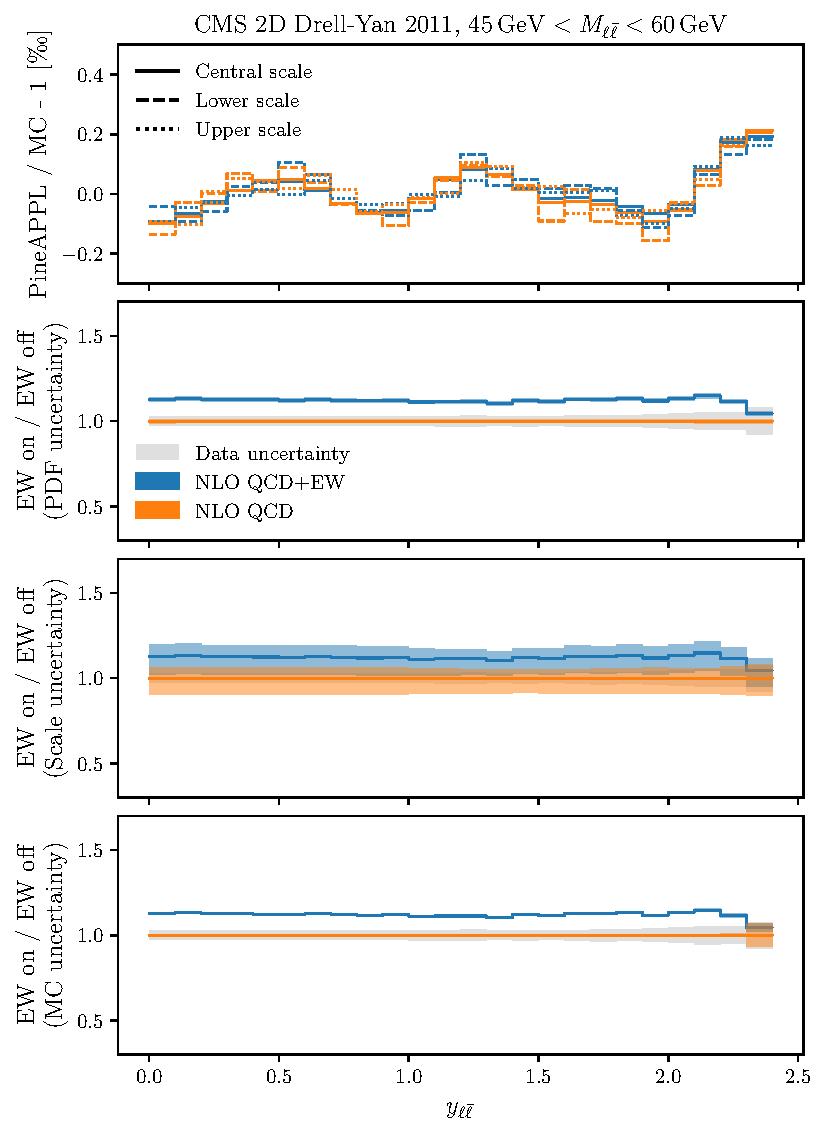
\includegraphics[width=0.5\textwidth]{figures/pineappl_CMSDY2D11_bin3}%
    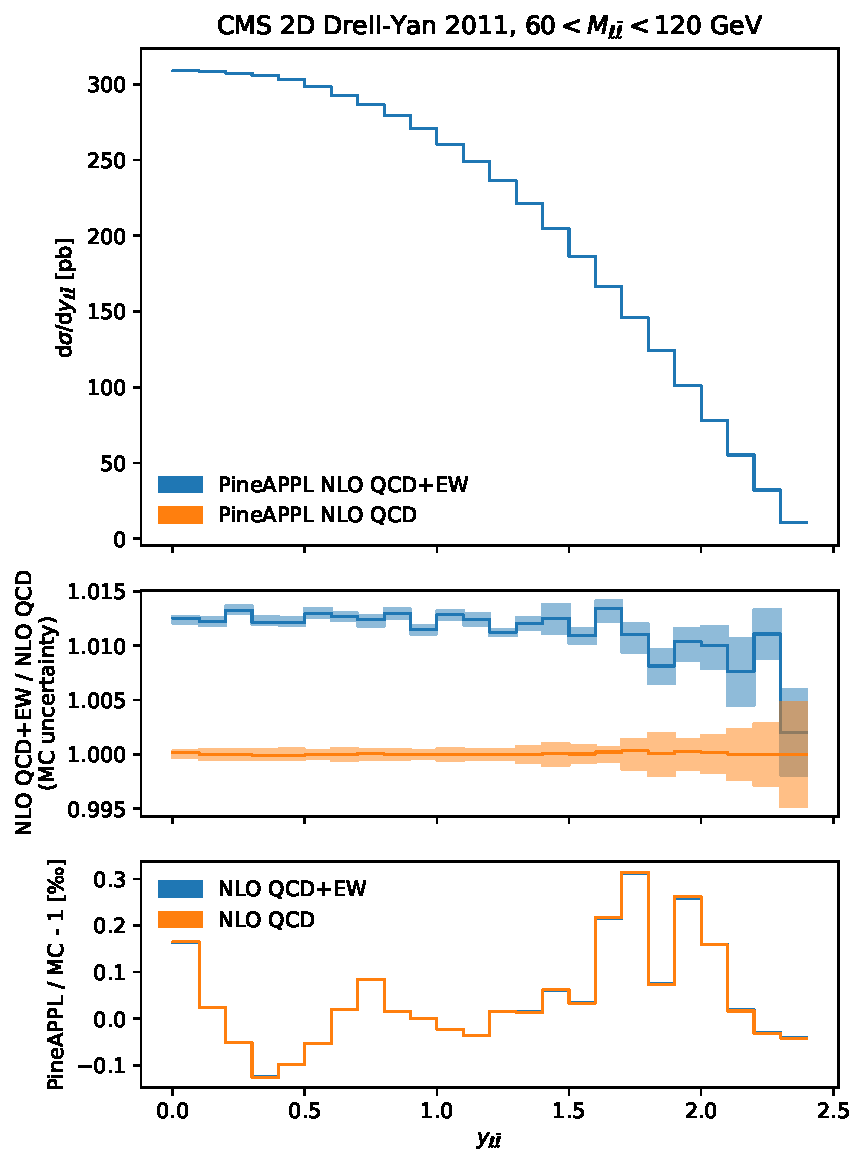
\includegraphics[width=0.5\textwidth]{figures/pineappl_CMSDY2D11_bin4}\\
    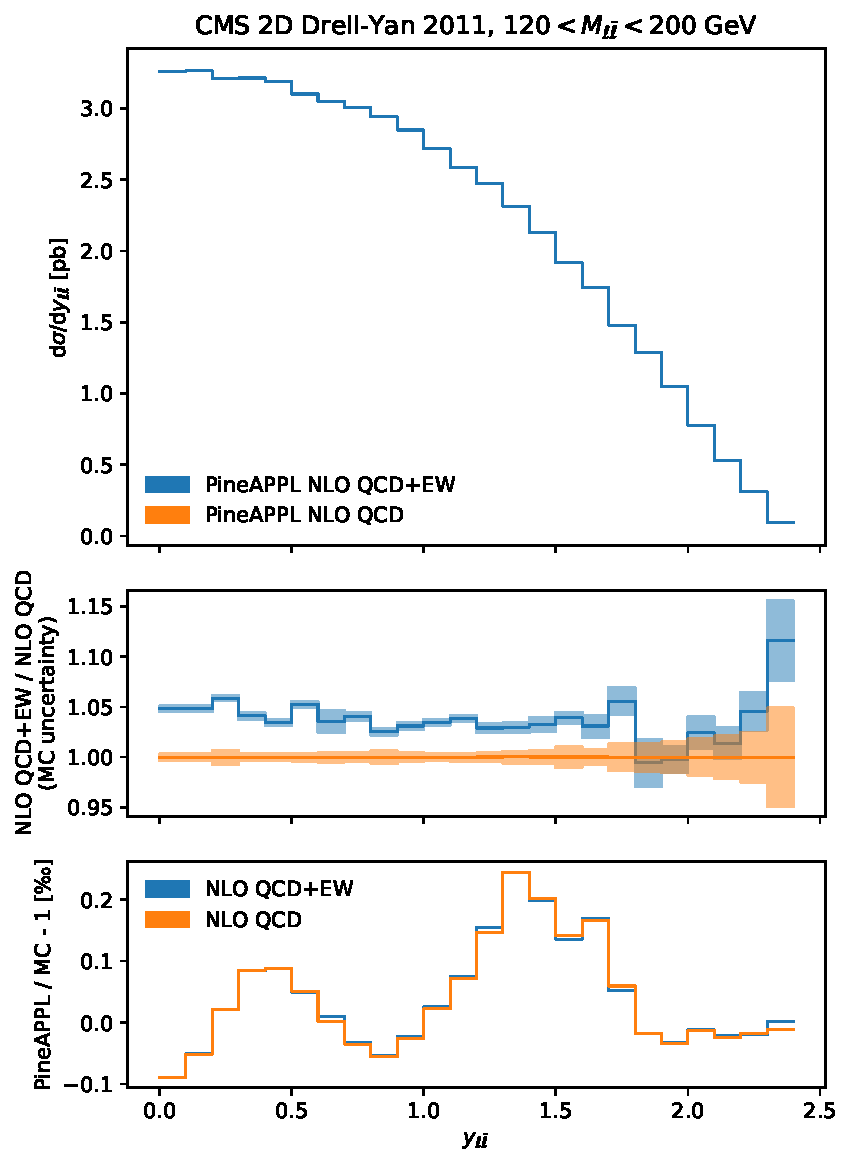
\includegraphics[width=0.5\textwidth]{figures/pineappl_CMSDY2D11_bin5}%
    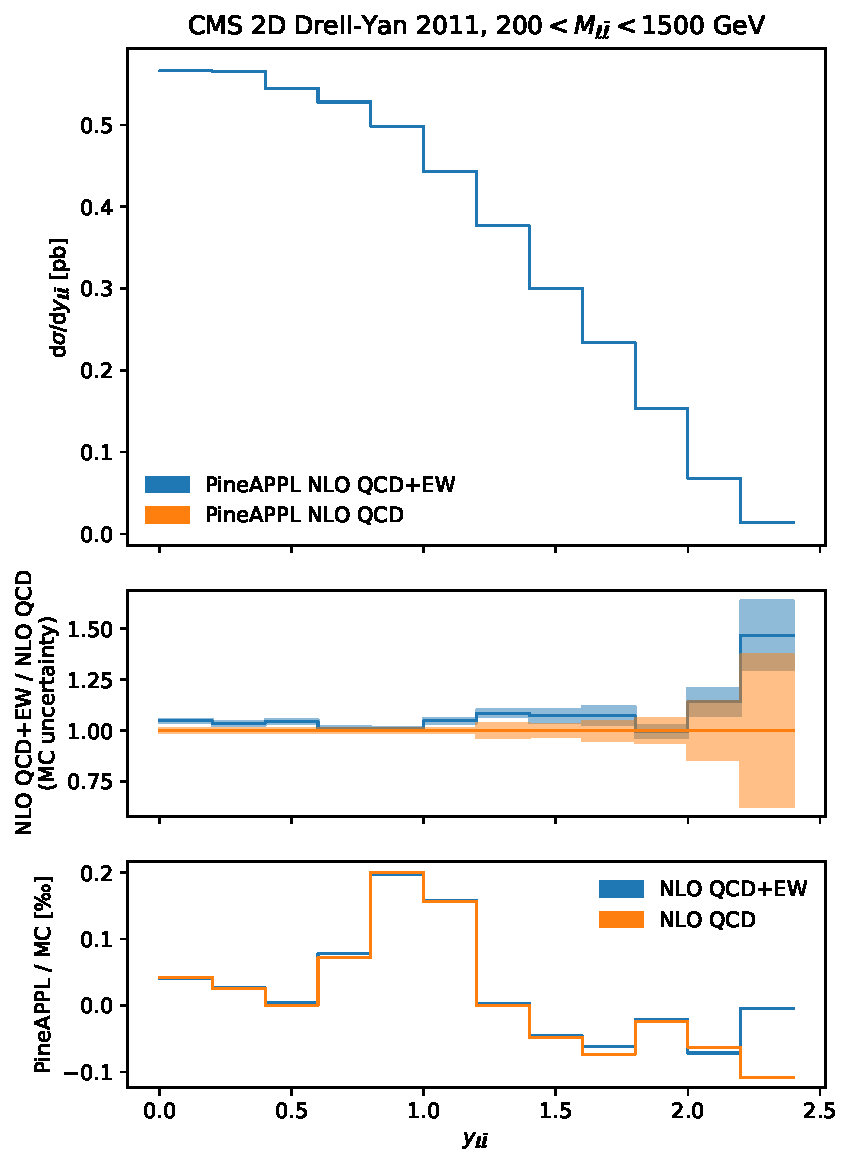
\includegraphics[width=0.5\textwidth]{figures/pineappl_CMSDY2D11_bin6}\\
    \caption{Same as figure~\ref{fig:atlaszhighmass49fb}, but for the CMS
      double-differential Drell--Yan lepton pair measurement at a
      centre-of-mass energy of \SI{7}{\tera\electronvolt}~\cite{Chatrchyan:2013tia}. Displayed are
      only two of the six invariant mass bins available, respectively below the
      Z-boson mass peak, $\SI{45}{\giga\electronvolt}<M_{\ell\bar\ell}<\SI{60}{\giga\electronvolt}$, on the Z-boson mass
      peak, $\SI{60}{\giga\electronvolt}<M_{\ell\bar\ell}<\SI{120}{\giga\electronvolt}$, above the mass peak,
      $\SI{120}{\giga\electronvolt}<M_{\ell\bar\ell}<\SI{200}{\giga\electronvolt}$, and at very high invariant masses,
      $\SI{200}{\giga\electronvolt}<M_{\ell\bar\ell}<\SI{1500}{\giga\electronvolt}$.}
    \label{fig:cmsdy2d11_bins3456}
\end{figure}
%-------------------------------------------------------------------------------

As in the case of the ATLAS high-mass Drell--Yan measurement, the CMS
measurement is also dominated by $\mathrm{q}\bar{\mathrm{q}}$ scattering. The leading
(next-to-leading) contribution to the $\SI{45}{\giga\electronvolt}<M_{\ell\bar\ell}<\SI{60}{\giga\electronvolt}$ invariant
mass bin comes from
the $\mathrm{u}\bar{\mathrm{u}}$ ($\mathrm{d}\bar{\mathrm{d}}$) parton luminosity, which accounts for about \SI{70}{\percent}
(\SI{22}{\percent}) of the double differential cross section, with small fluctuations across
the rapidity range. The PI contribution decreases from about \SI{4}{\percent} at zero
rapidity to \SI{1.5}{\percent} in the largest rapidity bin. The situation is slightly
different in the $\SI{60}{\giga\electronvolt}<M_{\ell\bar\ell}<\SI{120}{\giga\electronvolt}$ invariant mass bin, where the
leading (next-to-leading) contribution comes instead from the $\mathrm{d}\bar{\mathrm{d}}$
($\mathrm{u}\bar{\mathrm{u}}$) parton luminosity, which accounts for about \SI{60}{\percent} (\SI{44}{\percent}) of the
double differential cross section at small rapidities, and for about \SI{56}{\percent} (\SI{50}{\percent})
at large rapidities. In the remaining two invariant mass bins, the leading
(next-to-leading) contribution comes again from the $\mathrm{u}\bar{\mathrm{u}}$ ($\mathrm{d}\bar{\mathrm{d}}$)
parton luminosity, which accounts for about \SIrange{69}{95}{\percent} (\SIrange{38}{30}{\percent}) and
\SIrange{57}{70}{\percent} (\SIrange{48}{34}{\percent}) of the cross section, respectively for
$\SI{120}{\giga\electronvolt}<M_{\ell\bar\ell}<\SI{200}{\giga\electronvolt}$ and $\SI{200}{\giga\electronvolt}<M_{\ell\bar\ell}<\SI{1500}{\giga\electronvolt}$ in the
corresponding rapidity intervals; PI contributions range between \SIrange{7.3}{1.2}{\percent}
and \SIrange{3.7}{0.6}{\percent} in the two invariant mass bins, respectively, for increasing
rapidity.

The way in which NLO QCD+EW corrections affect the theoretical prediction for
the double differential cross section (with respect to its counterpart accurate
to NLO QCD) depends on the invariant mass bin. In the
$\SI{45}{\giga\electronvolt}<M_{\ell\bar\ell}<\SI{60}{\giga\electronvolt}$ region, they enhance the value of the cross
section by about \SI{11}{\percent} across all the rapidity range; in the
$\SI{60}{\giga\electronvolt}<M_{\ell\bar\ell}<\SI{120}{\giga\electronvolt}$ region, they suppress the value of the cross
section by about \SI{2}{\percent}, again across all the rapidity range; in the
$\SI{120}{\giga\electronvolt}<M_{\ell\bar\ell}<\SI{200}{\giga\electronvolt}$ bin, the suppression is around \SIrange{4}{5}{\percent}; and in
the $\SI{200}{\giga\electronvolt}<M_{\ell\bar\ell}<\SI{1500}{\giga\electronvolt}$ bin, the suppression increases further to
about \SIrange{6}{7}{\percent} for rapidities $y_{\ell\bar\ell}<2.0$ and up to \SIrange{20}{40}{\percent} at forward
rapidities. For this reason, for instance, the data points with
$M_{\ell\bar\ell}>\SI{200}{\giga\electronvolt}$ and $y_{\ell\bar\ell}>2.2$ were not included in the
NNPDF3.1 analysis~\cite{Ball:2017nwa}.

In general, the size of the EW corrections is comparable to or slightly larger
than the data uncertainty, except for the invariant mass bin 
$\SI{45}{\giga\electronvolt}<M_{\ell\bar\ell}<\SI{60}{\giga\electronvolt}$, where the shift due to the EW correction
overshoots the data uncertainty by about a factor of ten, and at large
rapidities, where the shift due to the EW correction, although it can become
large, is always a fraction of the data uncertainty. As already observed in the
case of the ATLAS measurement, should EW corrections be included in a fit of
PDFs, the description of the precise bins in the low invariant mass range is
likely to benefit from the more accurate theory; furthermore, the kinematic cut
that excludes any data point at large invariant mass and/or rapidity can be
safely removed.

In comparison to the PDF uncertainty, the size of the EW corrections is always
larger. We therefore anticipate that, once included in a PDF fit, they would
recast the relative weight of each data set included in the fit, and possibly
lead to an improvement in their overall description. In comparison to the scale
uncertainty, the size of the EW correction is similar, except on the Z-boson
mass peak, $\SI{60}{\giga\electronvolt}<M_{\ell\bar\ell}<\SI{120}{\giga\electronvolt}$, where the scale uncertainty exceeds
the size of the EW correction by about a factor of five. These facts confirm,
as expected, that EW corrections are almost immaterial at the Z-boson mass
peak, but that NNLO QCD corrections are otherwise as relevant as NLO QCD+EW
corrections. Finally, the Monte Carlo statistical uncertainty remains negligible
in comparison to the data, PDF and scale uncertainties, and to the size of the
EW correction, except for a couple of bins at forward rapidity in the highest
invariant mass bins. Improving the Monte Carlo statistical precision will
require to generate an unrealistically large number of events; therefore, it
might be desirable to treat this uncertainty as an additional theoretical
uncertainty in the PDF fit~\cite{Ball:2018lag}.

\paragraph{Top-quark pair production.} We now consider the top-pair differential
distributions measured by the ATLAS and CMS experiments at
\SI{7}{\tera\electronvolt}. In figure~\ref{fig:atlastop} we report the
distributions differential in the transverse momentum of the top quark,
$p_\mathrm{T}^\mathrm{t}$, and in the invariant mass of the top-quark pair,
$m_{\mathrm{t}\bar{\mathrm{t}}}$. Analogous plots for the distributions differential
in the rapidity of either the top quark or the top-quark pair are collected in
appendix~\ref{app:add_plots}. From figure~\ref{fig:atlastop}, we immediately
validate the \textsc{PineAPPL} result: its relative difference with respect to
the MC result is at most as large as $0.4\tcperthousand$, irrespective of the
accuracy of the theory, of the choice of scale and of the distribution
considered.

%-------------------------------------------------------------------------------
\begin{figure}[!t]
    \centering
    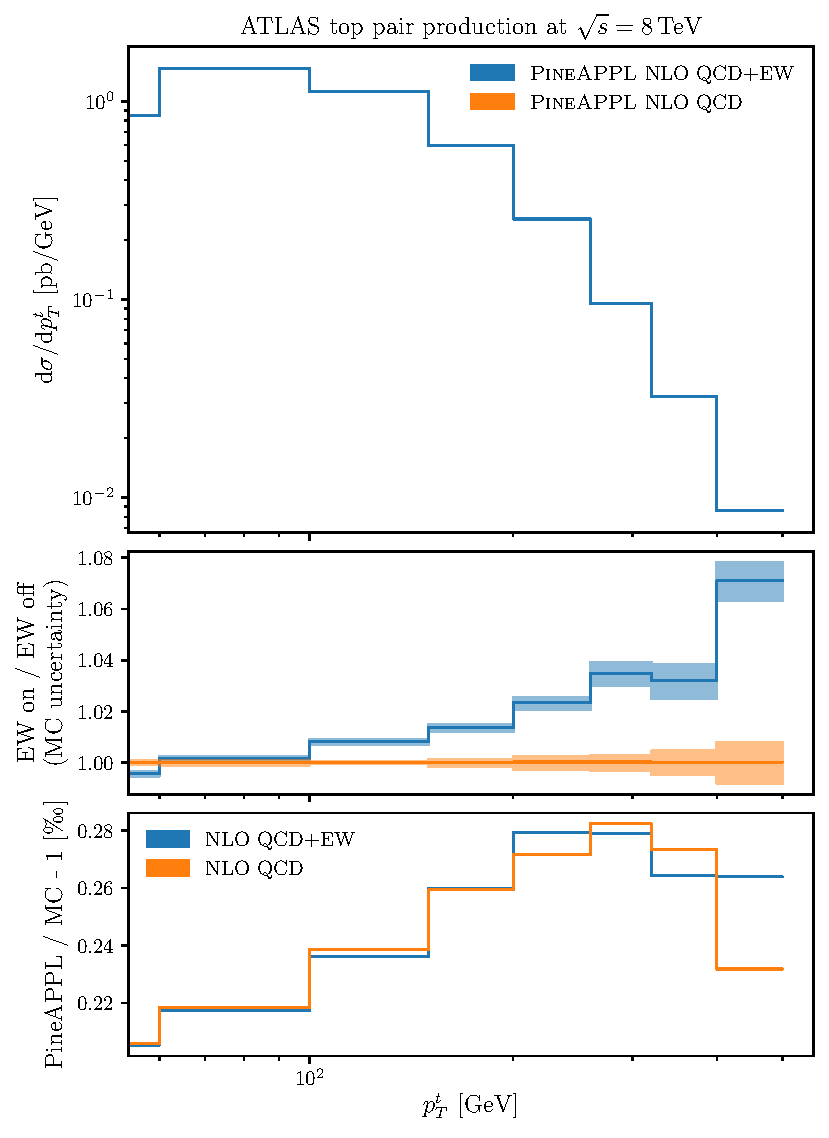
\includegraphics[width=0.5\textwidth]{figures/pineappl_ATLAS_TTB_DIFF_8TEV_LJ_TPT}%
    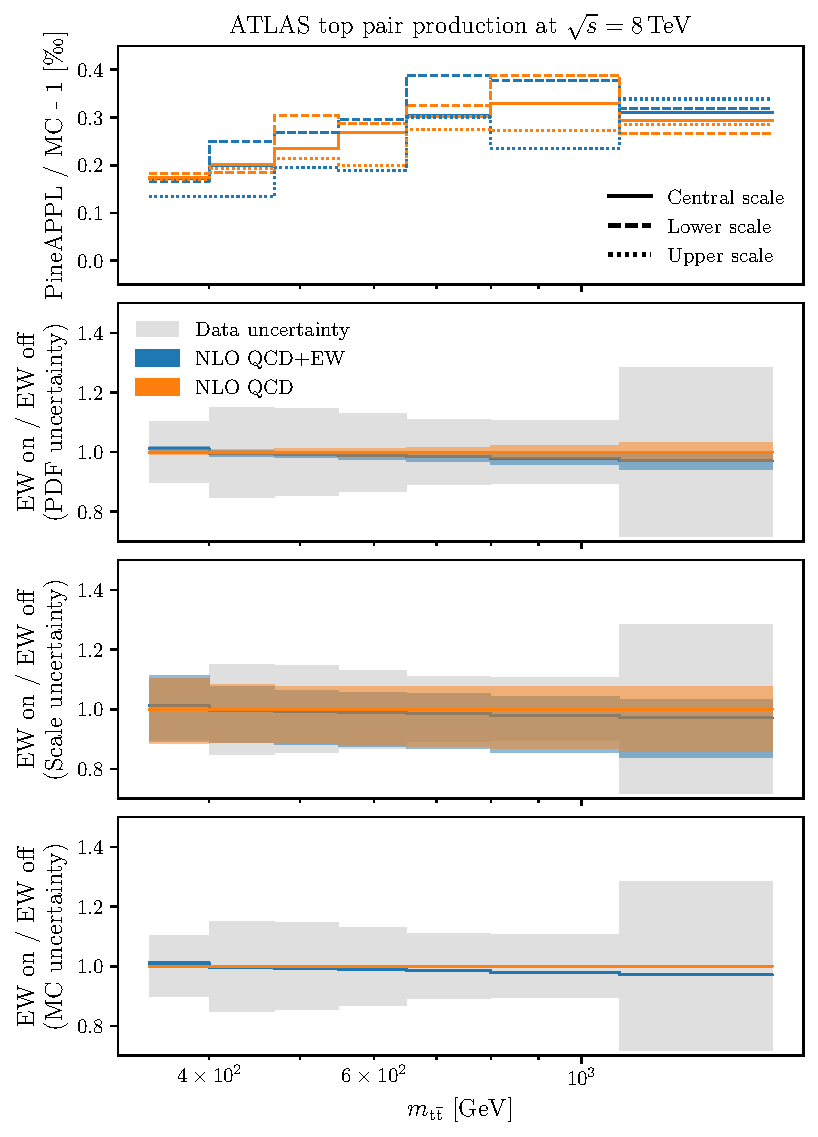
\includegraphics[width=0.5\textwidth]{figures/pineappl_ATLAS_TTB_DIFF_8TEV_LJ_TTM}
    \caption{Same as figure~\ref{fig:atlaszhighmass49fb}, but for the ATLAS
      differential top-quark pair measurement at a centre-of-mass energy of
      \SI{8}{\tera\electronvolt}~\cite{Aad:2015mbv}. Displayed are the distributions in the
      transverse momentum of the top quark $p_\mathrm{T}^\mathrm{t}$ (left), and in the invariant
      mass of the top-quark pair $m_{\mathrm{t}\bar{\mathrm{t}}}$ (right).}
    \label{fig:atlastop}
\end{figure}
%-------------------------------------------------------------------------------

The process is dominated by 

\paragraph{Z-boson production with non-zero transverse momentum.}


\begin{figure}[!t]
    \centering
    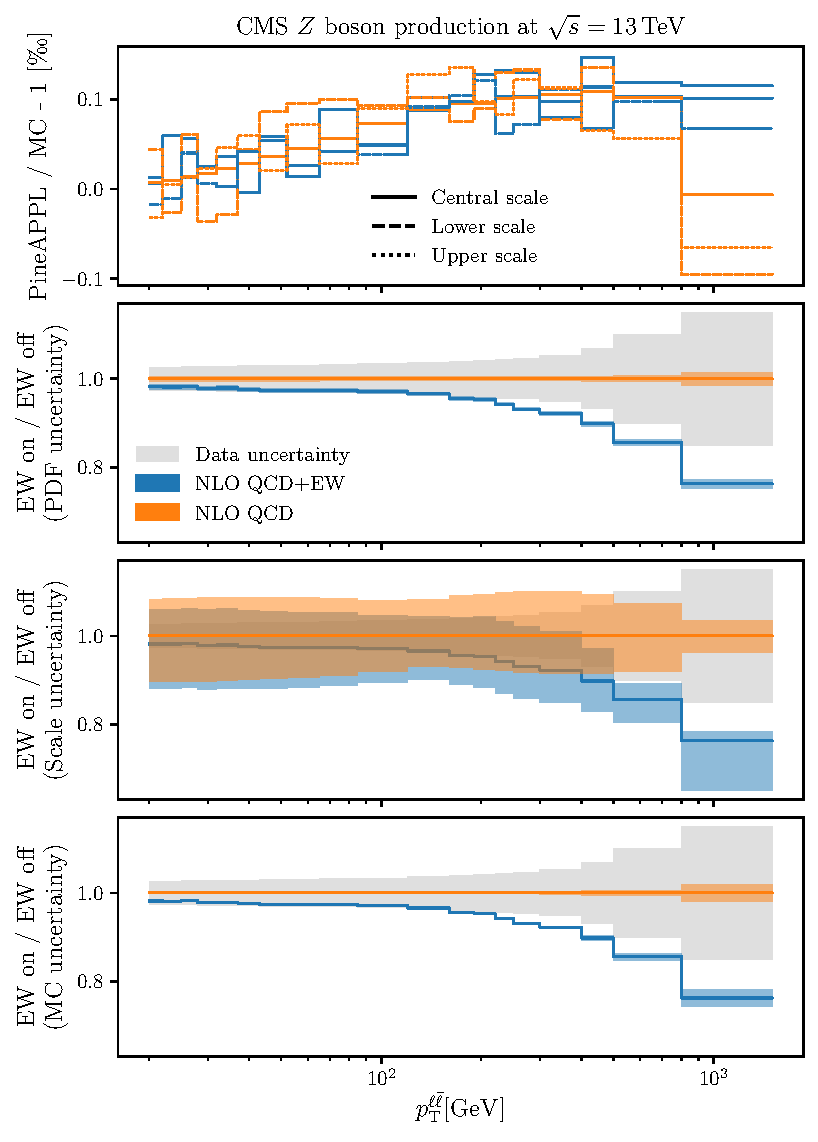
\includegraphics[width=0.5\textwidth]{figures/pineappl_CMS_Z_13_TEV}
    \caption{PineAPPL comparison for CMS Z $p_\mathrm{T}$ distribution.}
    \label{fig:cmsZ13TeV}
\end{figure}

